\documentclass[11pt]{beamer}
\usetheme{Boadilla}

\usepackage{agda}
\usepackage{tikz}
\usepackage{bbm}
\usepackage{animate}
\usepackage{hyperref}
\usepackage{graphicx}
\usepackage{longtable}
\usepackage{amsmath}
\usepackage{mdwlist}
\usepackage{txfonts}
\usepackage{xspace}
\usepackage{amstext}
\usepackage{amssymb}
\usepackage{stmaryrd}
\usepackage{proof}
\usepackage{multicol}
\usepackage[nodayofweek]{datetime}
\usepackage{etex}
\usepackage{textgreek}
\usepackage[all, cmtip]{xy}

\newcommand{\red}[1]{{\color{red}{#1}}}
\newcommand{\blue}[1]{{\color{blue}{#1}}}

\newenvironment{floatrule}
    {\hrule width \hsize height .33pt \vspace{.5pc}}
    {\par\addvspace{.5pc}}

\title{An Introduction to \\
Homotopy Type Theory}
\author{Amr Sabry}
\institute{
  School of Informatics and Computing \\
  Indiana University
}

\date{October 31, 2013} 

\begin{document}

\maketitle

\AgdaHide{
\begin{code}\>\<%
\\
\>\AgdaComment{-- \{-\# OPTIONS --without-K \#-\}}\<%
\\
\>\AgdaKeyword{module} \AgdaModule{talk3} \AgdaKeyword{where}\<%
\\
\>\AgdaKeyword{open} \AgdaKeyword{import} \AgdaModule{Data.Empty}\<%
\\
\>\AgdaKeyword{open} \AgdaKeyword{import} \AgdaModule{Data.Unit}\<%
\\
\>\AgdaKeyword{open} \AgdaKeyword{import} \AgdaModule{Data.Nat}\<%
\\
\>\AgdaKeyword{open} \AgdaKeyword{import} \AgdaModule{Data.Sum}\<%
\\
\>\AgdaKeyword{open} \AgdaKeyword{import} \AgdaModule{Data.Product}\<%
\\
\>\AgdaKeyword{import} \AgdaModule{Level}\<%
\\
%
\\
\>\AgdaKeyword{data} \AgdaDatatype{\_≡\_} \AgdaSymbol{\{}\AgdaBound{A} \AgdaSymbol{:} \AgdaPrimitiveType{Set}\AgdaSymbol{\}} \AgdaSymbol{:} \AgdaSymbol{(}\AgdaBound{a} \AgdaBound{b} \AgdaSymbol{:} \AgdaBound{A}\AgdaSymbol{)} \AgdaSymbol{→} \AgdaPrimitiveType{Set} \AgdaKeyword{where}\<%
\\
\>[0]\AgdaIndent{2}{}\<[2]%
\>[2]\AgdaInductiveConstructor{refl} \AgdaSymbol{:} \AgdaSymbol{(}\AgdaBound{a} \AgdaSymbol{:} \AgdaBound{A}\AgdaSymbol{)} \AgdaSymbol{→} \AgdaSymbol{(}\AgdaBound{a} \AgdaDatatype{≡} \AgdaBound{a}\AgdaSymbol{)}\<%
\\
\>\<\end{code}
}

%%%%%%%%%%%%%%%%%%%%%%%%%%%%%%%%%%%%%%%%%%%%%%%%%%%%%%%%%%%%%%%%%%%%%%%%%
\begin{frame}{Higher-Order Inductive Types}
\begin{itemize}
\vfill\item We cannot generate non-trivial groupoids starting from the 
  usual type constructions;
\vfill\item We need \red{higher-order inductive types}
\vfill\item A \red{new} development (2012)
\vfill\item You specify not only the points in the ``set'' but also the 
  various (iterated) paths
\end{itemize}
\vfill
\end{frame}

%%%%%%%%%%%%%%%%%%%%%%%%%%%%%%%%%%%%%%%%%%%%%%%%%%%%%%%%%%%%%%%%%%%%%%%%%
\begin{frame}{Higher-Order Inductive Types (example)}

\begin{code}\>\<%
\\
\>\AgdaComment{-- data Circle : Set where}\<%
\\
\>\AgdaComment{--   base : Circle}\<%
\\
\>\AgdaComment{--   loop : base ≡ base}\<%
\\
%
\\
\>\AgdaKeyword{module} \AgdaModule{Circle} \AgdaKeyword{where}\<%
\\
\>[0]\AgdaIndent{2}{}\<[2]%
\>[2]\AgdaKeyword{private} \AgdaKeyword{data} \AgdaDatatype{S¹*} \AgdaSymbol{:} \AgdaPrimitiveType{Set} \AgdaKeyword{where} \AgdaInductiveConstructor{base*} \AgdaSymbol{:} \AgdaDatatype{S¹*}\<%
\\
%
\\
\>[0]\AgdaIndent{2}{}\<[2]%
\>[2]\AgdaFunction{S¹} \AgdaSymbol{:} \AgdaPrimitiveType{Set}\<%
\\
\>[0]\AgdaIndent{2}{}\<[2]%
\>[2]\AgdaFunction{S¹} \AgdaSymbol{=} \AgdaDatatype{S¹*}\<%
\\
%
\\
\>[0]\AgdaIndent{2}{}\<[2]%
\>[2]\AgdaFunction{base} \AgdaSymbol{:} \AgdaFunction{S¹}\<%
\\
\>[0]\AgdaIndent{2}{}\<[2]%
\>[2]\AgdaFunction{base} \AgdaSymbol{=} \AgdaInductiveConstructor{base*}\<%
\\
%
\\
\>[0]\AgdaIndent{2}{}\<[2]%
\>[2]\AgdaKeyword{postulate} \AgdaPostulate{loop} \AgdaSymbol{:} \AgdaFunction{base} \AgdaDatatype{≡} \AgdaFunction{base}\<%
\\
\>\<\end{code}

\end{frame}

%%%%%%%%%%%%%%%%%%%%%%%%%%%%%%%%%%%%%%%%%%%%%%%%%%%%%%%%%%%%%%%%%%%%%%%%%
\begin{frame}{Non-trivial structure of this example}

\begin{center}
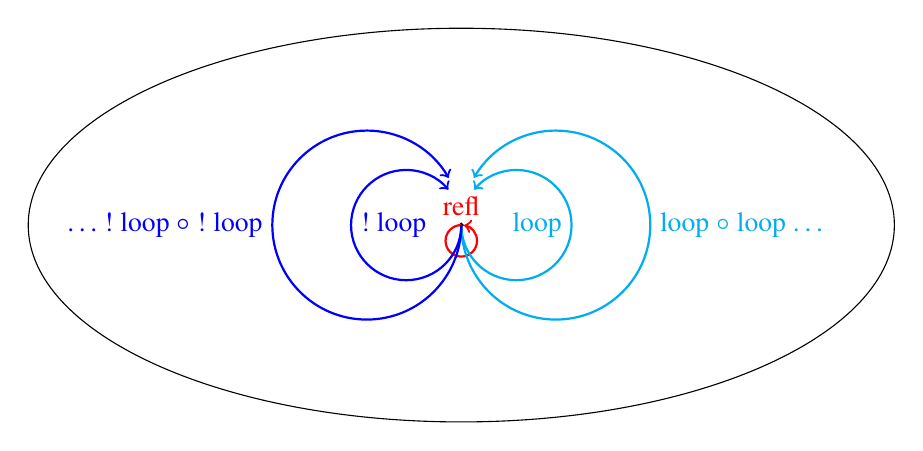
\begin{tikzpicture}
  \draw (0,0) ellipse (5.5cm and 2.5cm);
  \draw[fill] (0,0) circle [radius=0.025];
  \draw[->,thick,red] (0,0) arc (90:440:0.2);
  \node[above,red] at (0,0) {refl};
  \draw[->,thick,cyan] (0,0) arc (-180:140:0.7);
  \draw[->,thick,cyan] (0,0) arc (-180:150:1.2);
  \node[left,cyan] at (1.4,0) {loop};
  \node[right,cyan] at (2.4,0) {loop $\circ$ loop $\ldots$};
  \draw[->,thick,blue] (0,0) arc (360:40:0.7);
  \draw[->,thick,blue] (0,0) arc (360:30:1.2);
  \node[right,blue] at (-1.4,0) {!~loop};
  \node[left,blue] at (-2.4,0) {$\ldots$ !~loop $\circ$ !~loop};
\end{tikzpicture}
\end{center}

\end{frame}

%%%%%%%%%%%%%%%%%%%%%%%%%%%%%%%%%%%%%%%%%%%%%%%%%%%%%%%%%%%%%%%%%%%%%%%%%
\begin{frame}{Functions as functors}

\begin{itemize}

\vfill\item A function from space $A$ to space $B$ must map the points of $A$
to the points of $B$ as usual but it must also \red{respect the path
structure}

\vfill\item Mathematically, this corresponds to saying that every function
respects equality;

\vfill\item Topologically, this corresponds to saying that every function is
\red{continuous}.

\end{itemize}
\vfill
\end{frame}

%%%%%%%%%%%%%%%%%%%%%%%%%%%%%%%%%%%%%%%%%%%%%%%%%%%%%%%%%%%%%%%%%%%%%%%%%
\begin{frame}{Functions as functors}

\begin{center}
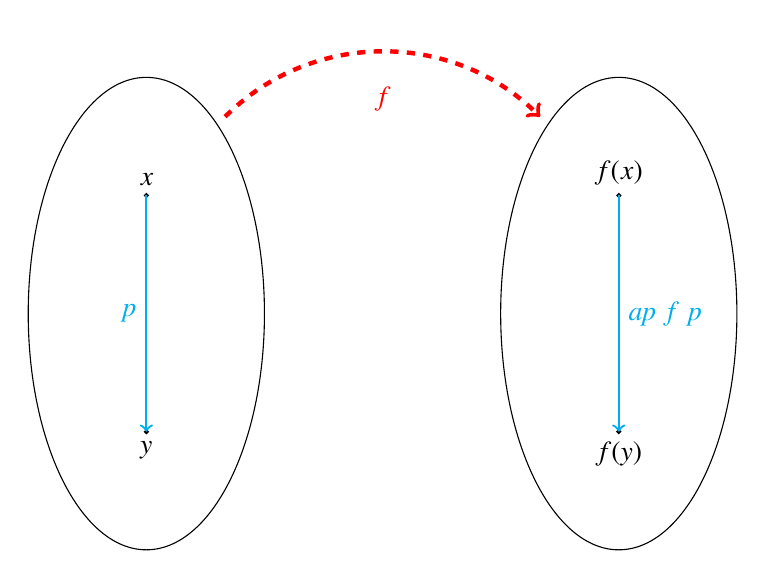
\begin{tikzpicture}
  \draw (-3,0) ellipse (1.5cm and 3cm);
  \draw (3,0) ellipse (1.5cm and 3cm);
  \draw[fill] (-3,1.5) circle [radius=0.025];
  \draw[fill] (-3,-1.5) circle [radius=0.025];
  \node[above] at (-3,1.5) {$x$};
  \node[below] at (-3,-1.5) {$y$};
  \draw[fill] (3,1.5) circle [radius=0.025];
  \draw[fill] (3,-1.5) circle [radius=0.025];
  \node[above] at (3,1.5) {$f(x)$};
  \node[below] at (3,-1.5) {$f(y)$};
  \draw[->,cyan,thick] (-3,1.5) -- (-3,-1.5);
  \node[left,cyan] at (-3,0) {$p$};
  \draw[->,cyan,thick] (3,1.5) -- (3,-1.5);
  \node[right,cyan] at (3,0) {$\mathit{ap}~f~p$};
  \draw[->,red,dashed,ultra thick] (-2,2.5) to [out=45, in=135] (2,2.5);
  \node[red,below] at (0,3) {$f$};
\end{tikzpicture}
\end{center}

\end{frame}

%%%%%%%%%%%%%%%%%%%%%%%%%%%%%%%%%%%%%%%%%%%%%%%%%%%%%%%%%%%%%%%%%%%%%%%%%
\begin{frame}{Functions as functors}

\begin{itemize}
\vfill\item \blue{$\mathit{ap}~f~p$} is the \red{action of $f$ on a path $p$};
\vfill\item This satisfies the following properties:
  \begin{itemize}
  \vfill\item $\mathit{ap}~f~(p \circ q) \equiv 
                (\mathit{ap}~f~p) \circ (\mathit{ap}~f~q)$;
  \vfill\item $\mathit{ap}~f~(!~p) \equiv ~!~(\mathit{ap}~f~p)$;
  \vfill\item $\mathit{ap}~g~(\mathit{ap}~f~p) \equiv 
                \mathit{ap}~(g \circ f)~p$;
  \vfill\item $\mathit{ap}~\mathit{id}~p \equiv p$.
  \end{itemize}
\end{itemize}
\vfill
\end{frame}

%%%%%%%%%%%%%%%%%%%%%%%%%%%%%%%%%%%%%%%%%%%%%%%%%%%%%%%%%%%%%%%%%%%%%%%%%
\begin{frame}{Type families as fibrations}
\vfill
\begin{itemize}

\vfill\item A more complicated version of the previous idea for dependent
functions;

\vfill\item The problem is that for dependent functions $f(x)$ and $f(y)$ may
not be in the same type, i.e., they live in different spaces;

\vfill\item Idea is to \red{transport} $f(x)$ to the space of $f(y)$;

\vfill\item Because everything is ``continuous'', the path $p$ induces a
transport function that does the right thing.
\end{itemize}
\vfill
\end{frame}

%%%%%%%%%%%%%%%%%%%%%%%%%%%%%%%%%%%%%%%%%%%%%%%%%%%%%%%%%%%%%%%%%%%%%%%%%
\begin{frame}{Type families as fibrations}

\begin{center}
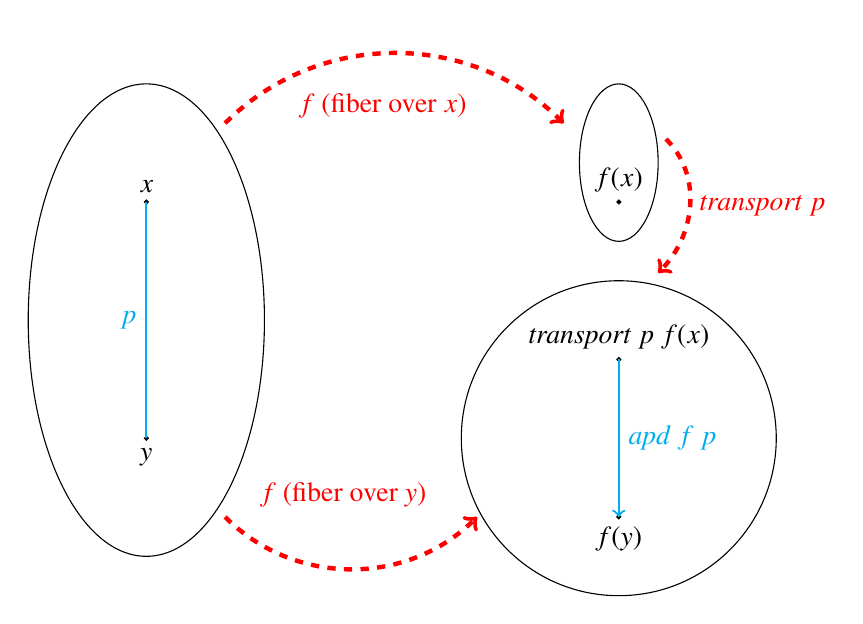
\begin{tikzpicture}
  \draw (-3,0) ellipse (1.5cm and 3cm);
  \draw (3,2) ellipse (0.5cm and 1cm);
  \draw (3,-1.5) ellipse (2cm and 2cm);
  \draw[fill] (-3,1.5) circle [radius=0.025];
  \draw[fill] (-3,-1.5) circle [radius=0.025];
  \node[above] at (-3,1.5) {$x$};
  \node[below] at (-3,-1.5) {$y$};
  \draw[fill] (3,1.5) circle [radius=0.025];
  \draw[fill] (3,-0.5) circle [radius=0.025];
  \draw[fill] (3,-2.5) circle [radius=0.025];
  \node[above] at (3,1.5) {$f(x)$};
  \node[above] at (3,-0.5) {$\mathit{transport}~p~f(x)$};
  \node[below] at (3,-2.5) {$f(y)$};
  \draw[left,cyan,thick] (-3,1.5) -- (-3,-1.5);
  \node[left,cyan] at (-3,0) {$p$};
  \draw[->,cyan,thick] (3,-0.5) -- (3,-2.5);
  \node[right,cyan] at (3,-1.5) {$\mathit{apd}~f~p$};
  \draw[->,red,dashed,ultra thick] (-2,2.5) to [out=45, in=135] (2.3,2.5);
  \node[red,below] at (0,3) {$f$ (fiber over $x$)};
  \draw[->,red,dashed,ultra thick] (-2,-2.5) to [out=-45, in=-135] (1.2,-2.5);
  \node[red,above] at (-0.5,-2.5) {$f$ (fiber over $y$)};
  \draw[->,red,dashed,ultra thick] (3.6,2.3) to [out=-45, in=45] (3.5,0.6);
  \node[red,right] at (3.9,1.45) {$\mathit{transport}~p$};
\end{tikzpicture}
\end{center}


\end{frame}

%%%%%%%%%%%%%%%%%%%%%%%%%%%%%%%%%%%%%%%%%%%%%%%%%%%%%%%%%%%%%%%%%%%%%%%%%
\begin{frame}{Extensional Equivalences}

\end{frame}

%%%%%%%%%%%%%%%%%%%%%%%%%%%%%%%%%%%%%%%%%%%%%%%%%%%%%%%%%%%%%%%%%%%%%%%%%
\begin{frame}{Univalence}

\end{frame}

%%%%%%%%%%%%%%%%%%%%%%%%%%%%%%%%%%%%%%%%%%%%%%%%%%%%%%%%%%%%%%%%%%%%%%%%%
\end{document}

